%=====================================================================
%  IT 7178 Research Progress: Implementation & Results  (IEEE conference)
%  Olaoluwa E. Sipeolu, Georgia Southern University
%
%  Self-contained version for Overleaf. Upload these three images to the
%  same project, with exactly these names:
%     fig_linux_graphs.png   fig_windows_graphs.png   fig_results.png
%  Compiler: pdfLaTeX (Overleaf default). No other files are needed.
%  The numbers below were generated by the executed notebook.
%=====================================================================
\documentclass[conference]{IEEEtran}
\IEEEoverridecommandlockouts
\usepackage{cite}
\usepackage{amsmath,amssymb}
\usepackage{graphicx}
\usepackage{url}
\usepackage{booktabs}
\usepackage{array}
% ---- numbers from the executed notebook ----
\newcommand{\LinTotal}{8}
\newcommand{\LinBenign}{5}
\newcommand{\LinMal}{3}
\newcommand{\LinHard}{0}
\newcommand{\LinTech}{3}
\newcommand{\LinBaseFP}{0}
\newcommand{\LinBaseFPR}{0.00}
\newcommand{\LinBasePrec}{1.00}
\newcommand{\LinBaseRec}{1.00}
\newcommand{\LinScoreFP}{0}
\newcommand{\LinScoreFPR}{0.00}
\newcommand{\LinScorePrec}{1.00}
\newcommand{\LinScoreRec}{1.00}
\newcommand{\LinScoreTwoRec}{0.33}
\newcommand{\LinAUC}{1.00}
\newcommand{\LinHardBase}{0}
\newcommand{\LinHardScore}{0}
\newcommand{\LinMissed}{none}
\newcommand{\LinMissedTwo}{\texttt{cron\_persist}, \texttt{download\_exec}}
\newcommand{\LinBaseMissed}{none}
\newcommand{\WinTotal}{54}
\newcommand{\WinBenign}{38}
\newcommand{\WinMal}{16}
\newcommand{\WinTech}{10}
\newcommand{\WinBaseFP}{2}
\newcommand{\WinBaseRec}{0.94}
\newcommand{\WinScoreFP}{1}
\newcommand{\WinScoreRec}{0.94}
\newcommand{\WinScoreTwoRec}{0.81}
\newcommand{\WinAUC}{0.96}
\newcommand{\LinuxFigCaption}{Linux process-provenance graphs. (a)--(c) benign administration; (d)--(f) emulated LotL techniques. Boxes are process executions; arrows point from parent to child.}

\begin{document}

\title{Behavior-Based Detection of Living-off-the-Land Attacks Using Process-Provenance Telemetry: Implementation and Preliminary Results}

\author{\IEEEauthorblockN{Olaoluwa E. Sipeolu}
\IEEEauthorblockA{\textit{M.S. Information Technology (Cybersecurity)}\\
\textit{Georgia Southern University}, Statesboro, GA, USA}}

\maketitle

\begin{abstract}
Living-off-the-Land (LotL) attacks misuse programs that already ship with
the operating system, such as PowerShell, WMI, certutil, bash, and curl.
Because no foreign malware is introduced, signature-based tools have little
to match, and rules written over command lines struggle because
administrators run the same programs every day. This progress report
examines whether the context in which a trusted binary runs (who launched
it, what it launched, and the chain it belongs to) separates malicious use
from routine administration. We implemented a pipeline that converts Linux
\texttt{auditd} and Windows Sysmon process-creation events into a common
process-provenance graph and scores each graph with interpretable behavioral
indicators mapped to MITRE ATT\&CK. The score is compared with a name-based
baseline that flags any well-known LotL binary. On an initial Linux lab
dataset of \LinTotal{} activities, both detectors classified every activity
correctly, which confirms the pipeline works but shows that the benign tasks
were too easy to separate the two approaches. On a Windows pilot built from
13 OTRF Security Datasets (\WinTotal{} execution units), the score reached a
ROC-AUC of \WinAUC{} and produced \WinScoreFP{} false positive against the
baseline's \WinBaseFP{}. The datasets are small and controlled, so these
results are preliminary; the next phase adds benign tasks that use the same
tools as the attacks and tests frozen indicators on unseen data.
\end{abstract}

\begin{IEEEkeywords}
Living-off-the-Land, process provenance, host-based intrusion detection, auditd, Sysmon, MITRE ATT\&CK
\end{IEEEkeywords}

%=====================================================================
\section{Introduction}
Modern adversaries increasingly avoid custom malware and instead ``live off
the land,'' repurposing legitimate operating-system utilities to conduct
reconnaissance, privilege escalation, and lateral movement. Because these
binaries are trusted and ubiquitous, allow-listing and signature matching
are ineffective, and the same tools are used constantly by legitimate
administrators, producing high false-positive rates for naive anomaly
detectors~\cite{barrsmith2021survivalism,ongun2021lotl}. The research gap is
a detection approach that reasons over the \emph{behavioral context} in
which a trusted binary executes rather than the binary or command in
isolation.

The question behind this work is simple to state. When an attacker and an
administrator run the same program, does the surrounding execution context
tell them apart more reliably than the program's name? To answer it, the
project has three objectives. The first is a provenance-graph representation
that works the same way for Linux and Windows telemetry. The second is a set
of behavioral indicators that an analyst can read and audit, each tied to a
MITRE ATT\&CK technique~\cite{strom2018attack}. The third is an evaluation
against a name-based baseline. The full evaluation needs benign activity
built from the same tools the attacks use, since that is where simple
detectors fail.

The problem matters in practice. Security teams already receive more alerts
than they can investigate, and false alarms on routine administration are a
large part of that load~\cite{hassan2019nodoze}. A detector that stays quiet
when an administrator runs \texttt{curl} or \texttt{crontab}, but not when
the same tools fetch and run a hidden payload, would reduce that noise
without giving up coverage.

Since the proposal, the project has moved from design to a working
implementation. This report describes the lab, the telemetry pipeline, the
indicator set, and first results on two datasets. Section~II reviews related
work, Section~III describes the implementation, Section~IV presents the
experiments and results, and Section~V summarizes progress and the plan for
the final paper.

%=====================================================================
\section{Literature Review}

\subsection{Scope}
The review covers two groups of work: detectors aimed specifically at LotL
and command-line abuse, and system-level provenance graphs for host intrusion
detection. Broader surveys of host-based and machine-learning intrusion
detection~\cite{bridges2019host,liu2019syscall,liao2013ids,buczak2016survey}
provide the context for both.

\subsection{LotL and Command-Line Detection}
Barr-Smith et al.~\cite{barrsmith2021survivalism} measured how Windows
malware uses built-in binaries and showed that the practice is widespread,
not limited to targeted attacks. Several detectors work directly on command
text. Hendler et al.~\cite{hendler2018powershell} trained deep neural
networks to classify PowerShell commands, and Outrata et al.~\cite{outrata2024obfuscation}
used small language models to recognize obfuscated command lines. Ongun et
al.~\cite{ongun2021lotl} applied active learning to command lines collected
from enterprise endpoints, which reduces the labeling effort but still
depends on analysts reviewing samples. These methods judge a command by its
text. They do not look at which process launched it or what it went on to
do, so a benign command and a malicious one that look alike are hard to
separate.

\subsection{Provenance-Graph Detection}
Provenance-based detection models a host as a graph of processes, files, and
network connections linked by causal events. King and
Chen~\cite{king2003backtracking} introduced backtracking over such
dependencies to trace intrusions to their source. SLEUTH~\cite{hossain2017sleuth}
and HOLMES~\cite{milajerdi2019holmes} reconstruct attack scenarios from
audit data in real time using tags and rules aligned with attacker
behavior, and POIROT~\cite{milajerdi2019poirot} searches audit graphs for
known attack patterns during threat hunting. A second line of work learns
what normal graphs look like. StreamSpot~\cite{manzoor2016streamspot},
UNICORN~\cite{han2020unicorn}, ProvDetector~\cite{wang2020provdetector}, and
Log2vec~\cite{liu2019log2vec} detect anomalies through graph sketches, rare
paths, or graph embeddings, and CONAN~\cite{xiong2022conan} uses a
state-based model for real-time APT detection. Other systems focus on the
analyst: NoDoze~\cite{hassan2019nodoze} and tactical provenance
analysis~\cite{hassan2020rapsheet} rank alerts by the rarity of their
context, while HERCULE~\cite{pei2016hercule} and
PrioTracker~\cite{liu2018priotracker} reconstruct attack stories from
correlated logs. Recent surveys~\cite{zipperle2023survey,li2021survey}
organize this area and its open problems.

\subsection{Critical Evaluation and Gap}
Command-only methods are lightweight but blind to context, so they tend to
flag administrators who use the same tools as attackers. Whole-system
provenance detectors capture that context, but they usually need
kernel-level collection of files and sockets as well as processes, large
amounts of training data, and considerable engineering, and their
evaluations rarely include benign use of the specific binaries that LotL
attacks rely on. Sommer and Paxson~\cite{sommer2010outside} also warned that
machine-learning intrusion detection is easy to evaluate optimistically,
which argues for transparent models and careful choice of negatives. What is
missing is a lighter approach in between: a provenance-aware score built
from process-creation events alone, readable by an analyst, usable on both
Linux and Windows, and tested against benign activity that looks like the
attacks. This project targets that gap.

%=====================================================================
\section{Research Implementation}

\subsection{Approach and Methodology}
\begin{table*}[!t]
\caption{Behavioral indicators $\phi_k$ and their platform-specific signals}
\label{tab:indicators}
\centering\footnotesize
\begin{tabular}{p{3.0cm}p{1.9cm}p{5.2cm}p{5.6cm}}
\toprule
\textbf{Concept} & \textbf{ATT\&CK} & \textbf{Linux (auditd) signal} & \textbf{Windows (Sysmon) signal}\\
\midrule
Decoded content to shell & T1140, T1027 & decoder (base64 -d, xxd -r, openssl -d, rev) sibling of a stdin shell & \texttt{-enc}/encoded token in a command line\\
Obfuscated command & T1027 & escape sequences, long hex/base64 tokens & script schemes (\texttt{javascript:}, \texttt{vbscript:}, \texttt{script:})\\
Remote / downloaded payload & T1105 & downloaded file later executed & URL or \texttt{/i:http} in a command line\\
Proxy / interpreter execution & T1218, T1059.006 & interpreter (python3, perl) spawns a shell & signed proxy LOLBin (mshta, regsvr32, cmstp, \dots); LOLBin spawns a child\\
Unusual execution context & T1047, T1548.002 & shell reading commands from a pipe & shell/admin tool with parent dllhost, WmiPrvSE, mshta, \dots\\
Execution from writable/hidden path & T1564.001, T1204 & image or script under /tmp, /dev/shm; hidden path; exec bit set there & image or payload under ProgramData, AppData, Temp\\
Persistence & T1053, T1546.004 & crontab install, shell-rc edit, systemctl enable & \texttt{schtasks /create}, Run key, \texttt{sc create}\\
Defense evasion & T1070.003, T1036.005, T1055 & history clearing; kernel-thread-like names & \texttt{mavinject /INJECTRUNNING}\\
Account manipulation & T1136 & (not used) & \texttt{net user /add}, admin group add\\
\bottomrule
\end{tabular}
\end{table*}

The working hypothesis is that malicious and benign use of the same trusted
binary differ in their provenance context: the parent that started the
process, the chain it belongs to, and what its command line asks it to do.
The pipeline has four stages. First, process-creation telemetry is captured
on the host. Second, the events for each activity are turned into a
provenance graph whose nodes are process executions and whose edges link a
parent to its child. Third, a set of behavioral indicators is evaluated on
the graph. Fourth, the graph receives a score equal to the number of
indicators that fire, as defined in~(\ref{eq:score}), and is flagged when
the score reaches a threshold. The indicators were written from ATT\&CK
technique descriptions and GTFOBins~\cite{gtfobins} entries rather than
learned from the data, which keeps every alert explainable.

\begin{equation}
S(G) \;=\; \sum_{k=1}^{K} \mathbb{1}\left[\,\phi_k(G)\,\right], \qquad \hat{y}(G) = \mathbb{1}\left[\,S(G) \ge \tau\,\right]
\label{eq:score}
\end{equation}
Here $G$ is the provenance graph of one activity, $\phi_k$ is the $k$-th
behavioral indicator (Table~\ref{tab:indicators}), and $\tau$ is the decision
threshold. The baseline flags $G$ if any process in it, other than the shell
that launched the activity, has a name on a list of well-known LotL
binaries.

\subsection{System and Workflow Design}
\begin{figure*}[!t]
\centering
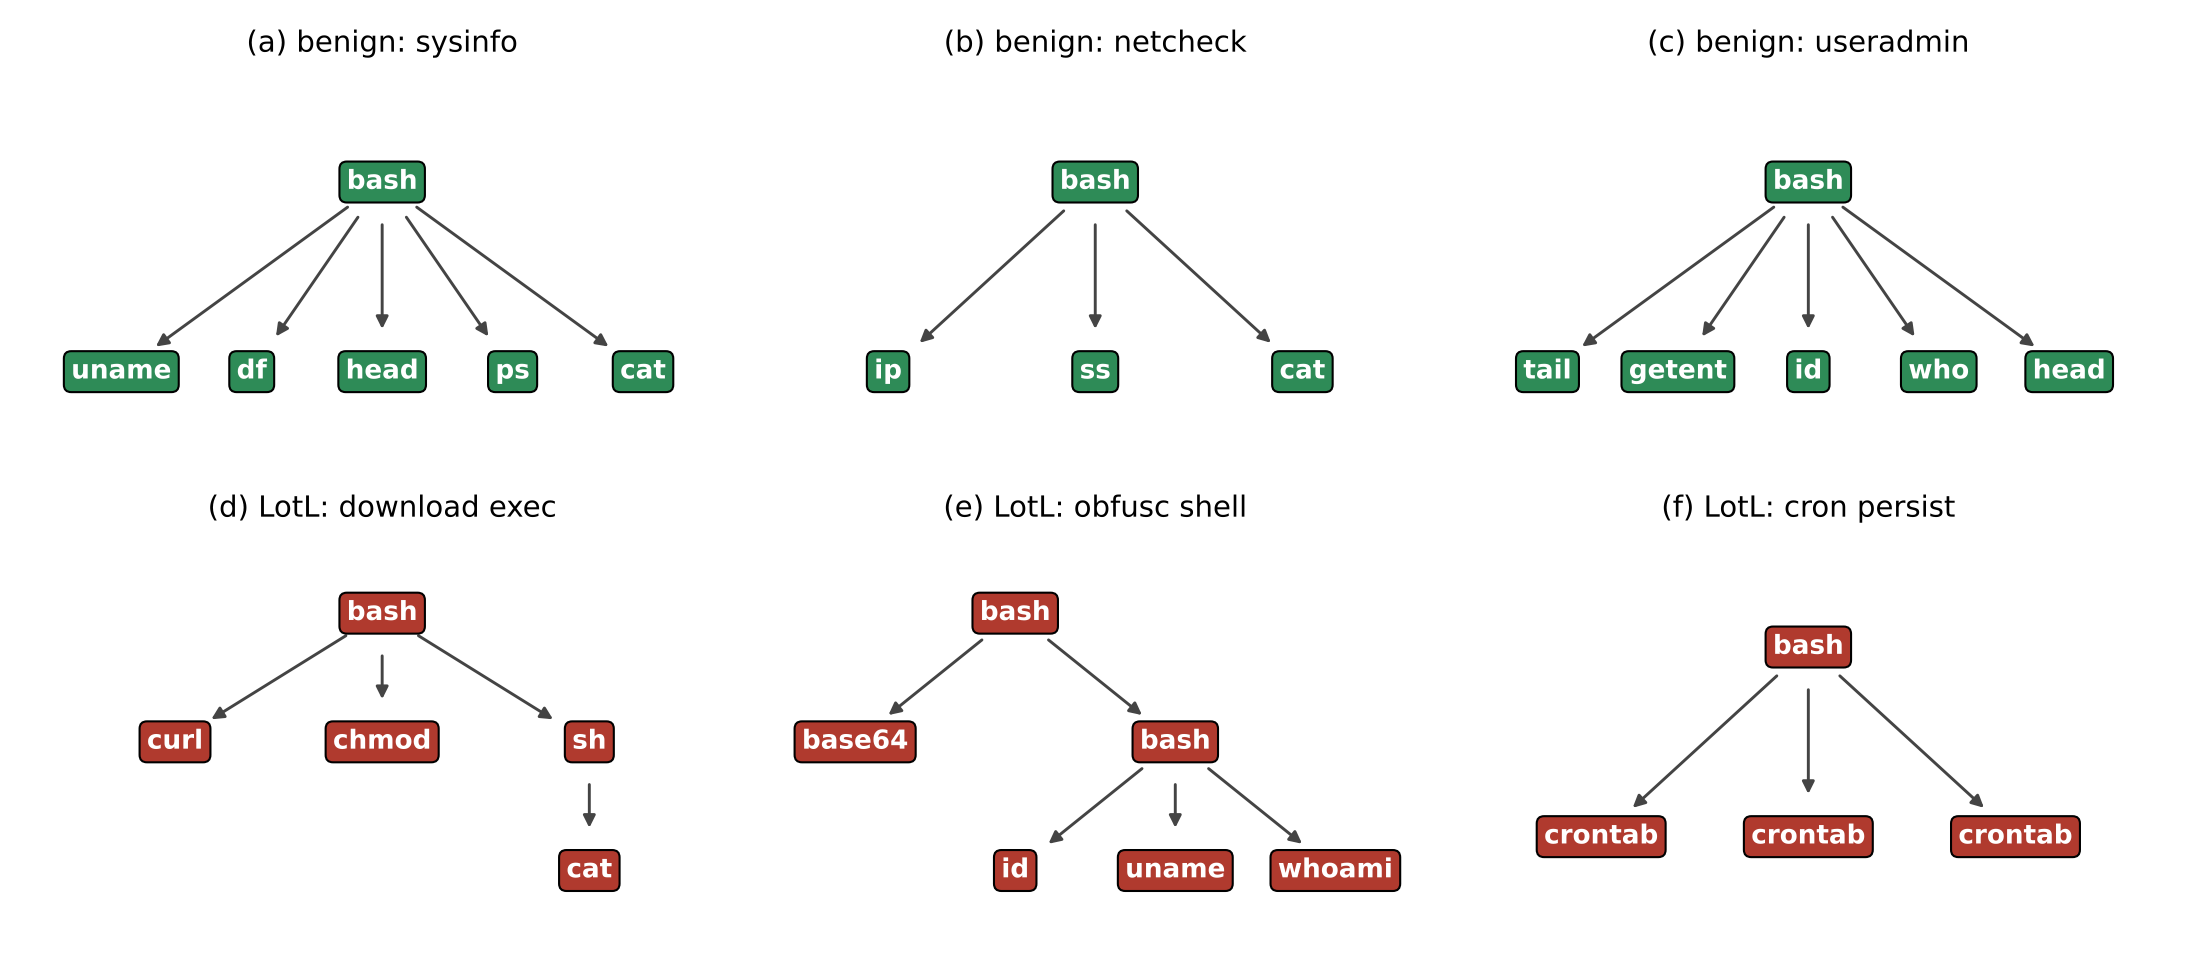
\includegraphics[width=\textwidth]{fig_linux_graphs.png}
\caption{\LinuxFigCaption}
\label{fig:linux}
\end{figure*}

\emph{Linux lab.} The lab runs Ubuntu Server 26.04 (ARM64) in a UTM virtual
machine on an Apple-silicon laptop. A kernel audit rule records every
program execution attempt, successful or not:
\begin{center}\small
\texttt{-a always,exit -F arch=b64 -S execve,execveat -k lotl\_exec}
\end{center}
A capture harness runs each labeled activity inside \texttt{bash -c}, waits
for it to finish, and saves the matching audit records to a file named after
the activity.

\emph{Graph construction (Linux).} Each successful \texttt{execve} becomes a
node with its process ID, image path, and full argument list. When a process
replaces its own image, as bash does when it runs the last command of a
script, the new execution keeps the same process ID; this is recorded as an
\emph{exec} edge so that a chain such as \texttt{bash}$\rightarrow$\texttt{sh}
is not lost. Every other process is linked to the most recent execution of
its parent process ID through a \emph{fork} edge. Failed \texttt{execve}
calls, which appear when a shell tries each directory on its search path,
are dropped. Finally, only the subtree under the activity's own
\texttt{bash -c} root is kept, which removes the harness and any unrelated
system activity from the graph.

\emph{Windows pilot.} Windows telemetry comes from Sysmon Event ID~1 in the
OTRF Security Datasets~\cite{otrf2020datasets}. Each event carries a
\texttt{ProcessGuid} and a \texttt{ParentProcessGuid}, which give the edges
directly. The unit of analysis is an \emph{execution unit}: a process whose
parent started before the recording began, together with all of its
descendants. The parent is kept as a context node because it is often the
most telling part of the chain, as with \texttt{WmiPrvSE} starting
\texttt{net.exe}. Parents are not shared between units, so long-running
system processes such as \texttt{services.exe} do not merge unrelated
activity into one graph. Fig.~\ref{fig:linux} and Fig.~\ref{fig:windows}
show example graphs from both platforms.

\begin{figure}[!t]
\centering
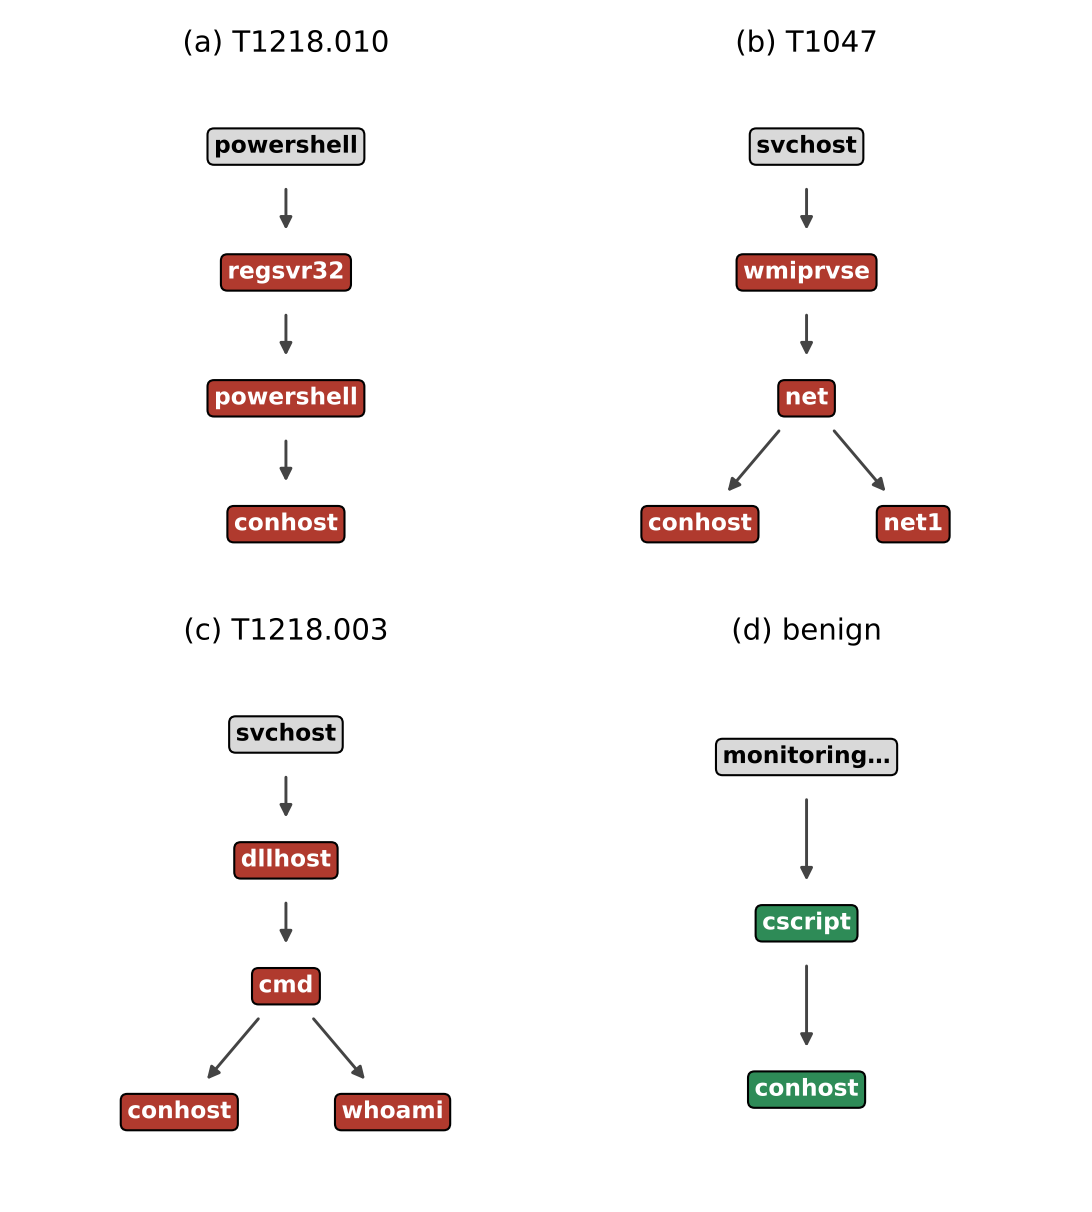
\includegraphics[width=\columnwidth]{fig_windows_graphs.png}
\caption{Windows execution units from OTRF; grey boxes are parents that started before the capture. (a) \texttt{regsvr32} proxy execution launching an encoded PowerShell stager; (b) WMI-spawned \texttt{net user /add}; (c) a CMSTP UAC bypass surfacing as \texttt{dllhost}$\rightarrow$\texttt{cmd}; (d) a benign monitoring agent running \texttt{cscript}, which the name-based baseline flags.}
\label{fig:windows}
\end{figure}

\subsection{Tools and Technologies}
Linux telemetry is collected with \texttt{auditd} and exported with
\texttt{ausearch}. Windows telemetry is taken from Sysmon logs in the OTRF
Security Datasets. Parsing, graph construction, and scoring are written in
Python using \texttt{networkx} for graphs, \texttt{pandas} for tabular data,
\texttt{scikit-learn} for metrics, and \texttt{matplotlib} for figures. The
analysis runs as a Google Colab notebook, and the code, audit rules, capture
scripts, and captured logs are in a public GitHub repository
(\url{https://github.com/os01752/lotl-provenance-detection}). The emulated
Linux techniques follow Atomic Red Team~\cite{atomicredteam} and
GTFOBins~\cite{gtfobins}. Every payload is harmless: it only runs commands
such as \texttt{id}, \texttt{whoami}, or \texttt{uname}, writes to
\texttt{/tmp} or the home directory, and removes its files afterward.

\subsection{Challenges Encountered}
Several practical problems shaped the implementation. The external SSD
intended for the virtual machine connected at USB~2.0 speed (about
38~MB/s for both reads and writes), so the VM was built on the internal
disk instead. The original plan favored eBPF tracing with Tracee, but on the
new ARM64 kernel (7.0) it was not practical to deploy in the time available,
so \texttt{auditd} was used because it works on any kernel and records the
fields the graphs need. Parsing turned out to be harder than expected:
\texttt{auditd} hex-encodes any argument that contains spaces, and two
details of process behavior, image replacement under the same PID and failed
lookups along the search path, initially produced wrong graphs until the
parser handled them. An early version of the baseline counted the
launching shell itself as a LotL binary, which inflated its false-positive
rate. Once that was fixed, it became clear that a fair comparison needs
benign tasks that use the same tools as the attacks, so a second capture
script with 41 more activities was written. Its first run produced empty
files: when \texttt{ausearch} is called from a script, it reads events from
standard input instead of the audit log unless \texttt{--input-logs} is
given. The script has been corrected and the set is being re-collected.
Finally, the Splunk Attack Data repository was considered
for external Linux data, but its \texttt{auditd} files keep only command
lines without process and parent IDs, so they cannot form provenance graphs.
The OTRF datasets, which keep full Sysmon process-creation events, were used
instead.

%=====================================================================
\section{Experimental Results}
\begin{figure*}[!t]
\centering
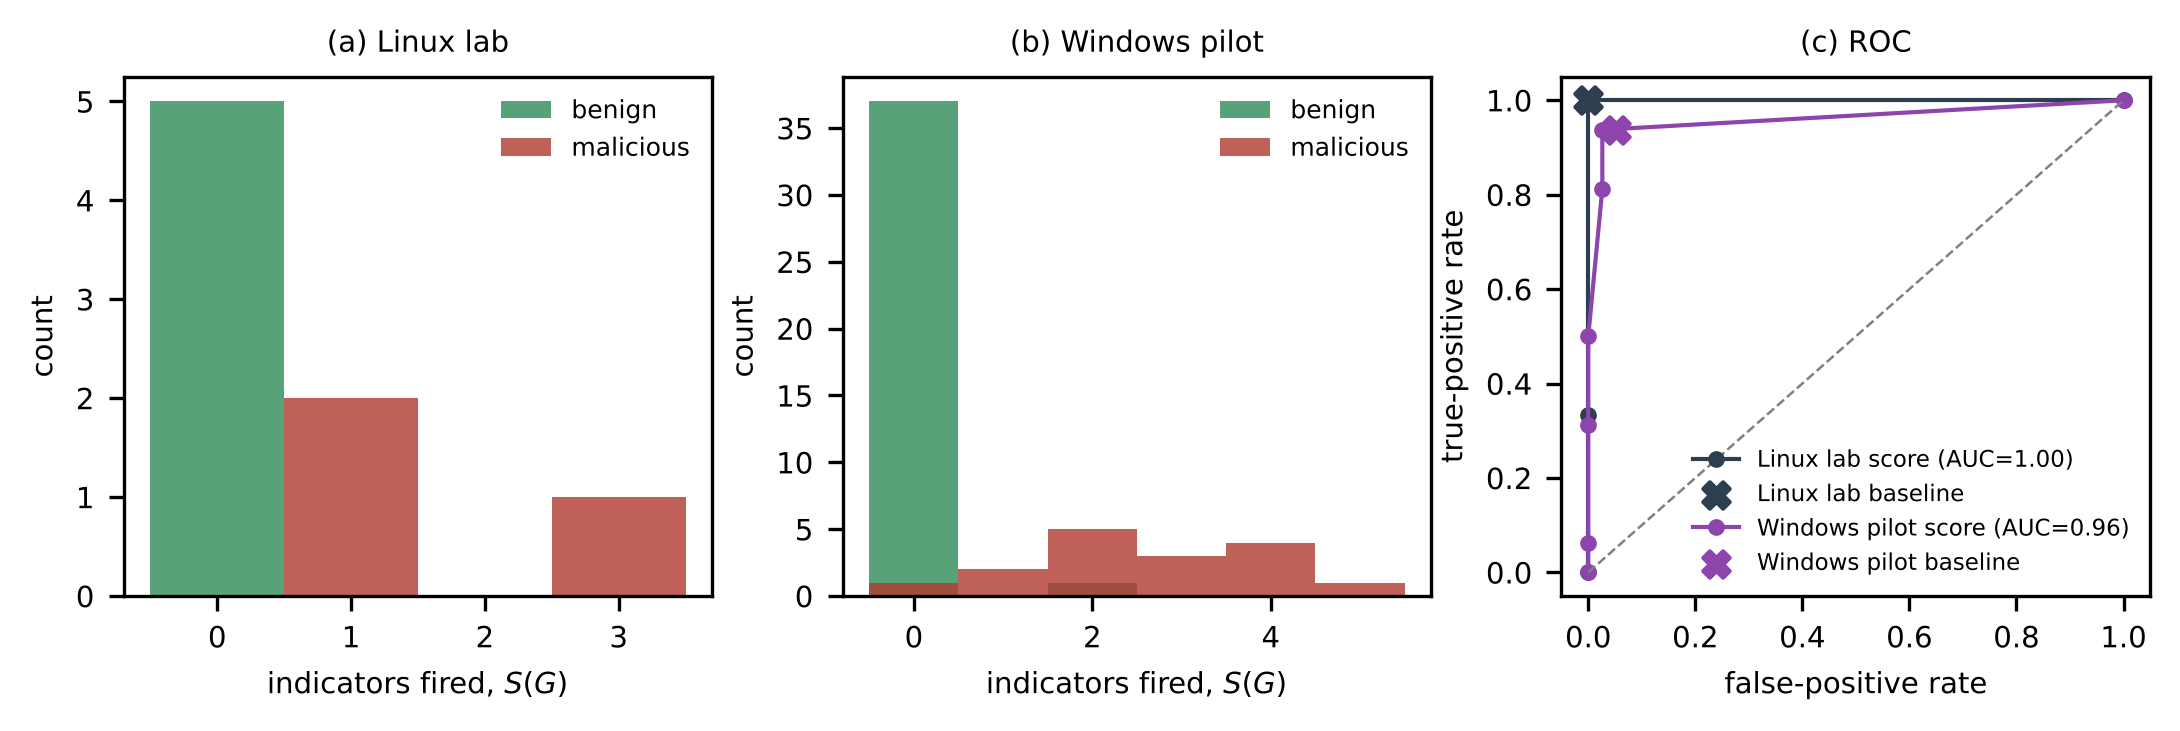
\includegraphics[width=\textwidth]{fig_results.png}
\caption{(a), (b) Distribution of the behavior score $S(G)$ for benign and malicious activity; (c) ROC curves of $S(G)$, with the name-based baseline's single operating point marked X.}
\label{fig:results}
\end{figure*}


\subsection{Experiment Setup}
\begin{table}[t]
\caption{Datasets}\label{tab:datasets}\centering\footnotesize
\resizebox{\columnwidth}{!}{\begin{tabular}{llrrr}\toprule
\textbf{Dataset} & \textbf{Unit} & \textbf{Benign} & \textbf{Malicious} & \textbf{ATT\&CK IDs}\\\midrule
Linux lab (auditd) & activity & 5 & 3 & 3\\
Windows pilot (OTRF Sysmon) & execution unit & 38 & 16 & 10\\
\bottomrule\end{tabular}}\end{table}
Table~\ref{tab:datasets} summarizes the two datasets. The Linux lab dataset
contains \LinTotal{} activities captured on the VM: \LinBenign{} benign
administrative tasks and \LinMal{} emulated LotL activities covering
\LinTech{} ATT\&CK techniques. The benign tasks are routine administration:
a system inventory (\texttt{uname}, \texttt{df}, \texttt{ps}), package
queries, a review of user accounts and logins, a log review, and a check of
network settings. The malicious activities are a Base64-encoded command
decoded and piped straight into \texttt{bash} (T1059.004), a file fetched
with \texttt{curl} into a hidden path under \texttt{/tmp} and made executable
(T1105), and a cron entry installed from a file in \texttt{/tmp}
(T1053.003). None of the benign tasks uses an attack-associated tool, which
is the main weakness of this first set and is addressed by the second
capture set described in Section~III-D.

The Windows pilot uses 13 OTRF datasets~\cite{otrf2020datasets}, each
recorded while one technique was executed on a lab domain. They contain
\WinTotal{} execution units, of which \WinMal{} belong to the documented
attacks (\WinTech{} techniques, including mshta, regsvr32, InstallUtil,
CMSTP, WMI, BITS, and scheduled tasks) and \WinBenign{} are normal background
activity of the same hosts. A unit is labeled malicious when it contains the
technique documented for its dataset. Units that only reflect a side effect
of the payload (the Windows Calculator app starting after \texttt{calc.exe})
were excluded. The Windows indicator vocabulary was written after these 13
files had been inspected, so this experiment is a feasibility pilot rather
than an unbiased test; the final paper will freeze the indicators and
evaluate them on OTRF datasets that have not been examined.

\subsection{Performance Metrics}
Counting $TP$, $FP$, $FN$, and $TN$ per activity (Linux) or per execution
unit (Windows), we report
\begin{equation}
P=\frac{TP}{TP+FP},\qquad R=\frac{TP}{TP+FN},
\end{equation}
\begin{equation}
F_1=\frac{2PR}{P+R},\qquad \mathit{FPR}=\frac{FP}{FP+TN}.
\end{equation}
The threshold $\tau$ is not learned, so results are given for $\tau=1$ and
$\tau=2$, together with the ROC-AUC of $S(G)$, which does not depend on a
threshold. The false-positive rate gets particular attention because false
alarms on administration are the problem this work addresses.

\subsection{Results Presentation}
\begin{table}[t]
\caption{Detection performance: name-based baseline vs. provenance behaviour score}\label{tab:results}
\centering\footnotesize\setlength{\tabcolsep}{3.5pt}
\resizebox{\columnwidth}{!}{\begin{tabular}{lccccc}\toprule
\textbf{Detector} & \textbf{P} & \textbf{R} & \textbf{F$_1$} & \textbf{FPR} & \textbf{TP/FP/FN/TN}\\\midrule
\multicolumn{6}{l}{\textit{Linux lab} (ROC-AUC of score = 1.000)}\\
\quad Name-based baseline & 1.000 & 1.000 & 1.000 & 0.000 & 3/0/0/5\\
\quad Provenance score $\ge$ 1 & 1.000 & 1.000 & 1.000 & 0.000 & 3/0/0/5\\
\quad Provenance score $\ge$ 2 & 1.000 & 0.333 & 0.500 & 0.000 & 1/0/2/5\\
\multicolumn{6}{l}{\textit{Windows pilot} (ROC-AUC of score = 0.961)}\\
\quad Name-based baseline & 0.882 & 0.938 & 0.909 & 0.053 & 15/2/1/36\\
\quad Provenance score $\ge$ 1 & 0.938 & 0.938 & 0.938 & 0.026 & 15/1/1/37\\
\quad Provenance score $\ge$ 2 & 0.929 & 0.812 & 0.867 & 0.026 & 13/1/3/37\\
\bottomrule\end{tabular}}\end{table}
Table~\ref{tab:results} gives the detection results for both datasets.
Fig.~\ref{fig:results} shows how the score is distributed for benign and
malicious activity and where the baseline sits relative to the score's ROC
curve. Fig.~\ref{fig:linux} and Fig.~\ref{fig:windows} show representative
graphs.

\subsection{Comparative Analysis}
On the Linux dataset both detectors classified all \LinTotal{} activities
correctly at $\tau=1$: recall \LinScoreRec{} and no false positives. This
tells us the pipeline and indicators work on real audit data, but it does not
favor either approach. The baseline succeeds only because none of the benign
tasks touches \texttt{curl}, \texttt{chmod}, \texttt{base64}, or
\texttt{crontab}; once an administrator uses those tools, a name list has no
way to tell the two apart. Raising the threshold to $\tau=2$ dropped Linux
recall to \LinScoreTwoRec{}, because the cron and download emulations each
trigger a single indicator (persistence, and an execute bit set on a hidden
file in \texttt{/tmp}), while the encoded-shell emulation triggers three.

The Windows pilot is where the two detectors first differ. The baseline
produced \WinBaseFP{} false positives, both from a Microsoft monitoring agent
that runs \texttt{cscript.exe} for routine checks, while the score produced
\WinScoreFP{}. Both reached a recall of \WinScoreRec{}. The difference is
modest because the benign units in OTRF are mostly Windows services starting
helper processes, which rarely involve LotL binaries at all. On Windows, too,
raising the threshold to $\tau=2$ lowered recall (to \WinScoreTwoRec{})
without removing the remaining false positive, so $\tau=1$ is the better
operating point on the current data. The threshold will be chosen on
held-out data in the final evaluation.

\subsection{Interpretation of Results}
The Linux graphs show the structure the method relies on
(Fig.~\ref{fig:linux}). Every benign task is shallow: one shell starts a few
ordinary utilities, and at most one of them starts a helper of its own (for
example, \texttt{dpkg} calling \texttt{dpkg-query}). The encoded-shell attack
looks different even though it starts from the same shell, because a
\texttt{base64} decoder and a second \texttt{bash} reading from a pipe sit
side by side under it, which is exactly the pattern the decode-to-shell
indicator looks for. The download emulation also exposed a weakness in the
test itself: it wrote and marked the payload executable but only read it
with \texttt{cat}, so the download-then-execute indicator correctly stayed
silent. The second capture set executes its payloads. The real test of the
hypothesis is benign work with the same tools. An administrator who
downloads a file with \texttt{curl} saves it in the home directory and reads
it; an attacker writes it to a hidden path in \texttt{/tmp}, sets the execute
bit, and runs it. The tool name is the same, but the provenance graph is
not, and the second capture set is designed around such pairs.

The two Windows errors are informative. The score's false positive is a
Windows Search helper whose command line contains long pipe names that look
like encoded data, which shows that the encoding indicator needs an
allow-list for known system formats. The one attack both detectors missed is
the \texttt{notepad.exe} process that \texttt{mavinject} injected into: on
its own, that process looks completely normal, and only the injector is
visible in process-creation events. Detecting it would require other event
types, such as Sysmon's process-access events. The pilot also suggests that
background noise on a Windows host is not the hard case; benign
administration with the same tools is, which is why the next Linux capture
focuses on it.

These results come with clear limits. Both datasets are small. On Linux, the
same person wrote the emulations and the indicators, which can make results
look better than they would on unfamiliar attacks. On Windows, the
indicators were written after the pilot files were inspected. The score also
gives every indicator equal weight. Together these limits mean the numbers
should be read as early evidence that the pipeline works, not as a measured
detection rate.

%=====================================================================
\section{Conclusion and Plan for the Final Paper}
The project now has a working pipeline that turns Linux \texttt{auditd} and
Windows Sysmon process-creation events into one provenance-graph format,
scores each graph with readable ATT\&CK-mapped indicators, and compares the
result with a name-based baseline. On the Windows pilot the score raised
fewer false alarms than the baseline, and on the initial Linux set both
detectors were correct on every activity, which shows that the Linux data
needs harder benign cases before it can separate them. The remaining work
for the final paper is as follows. First, the indicators will be frozen and
tested on OTRF datasets that were not used during development. Second, a
learned model (logistic regression and random forest on the indicator and
structural features) will be evaluated with cross-validation and
leave-one-technique-out splits. Third, the obfuscation-robustness experiment
from the proposal will test how the score holds up when attack commands are
rewritten. Fourth, the corrected second Linux capture set (41 more
activities, 12 of them benign tasks that use the same tools as the attacks)
will be collected, along with repeated runs, so that the Linux results can
test the hypothesis directly.

% Generated by IEEEtran.bst, version: 1.14 (2015/08/26)
\begin{thebibliography}{10}
\providecommand{\url}[1]{#1}
\csname url@samestyle\endcsname
\providecommand{\newblock}{\relax}
\providecommand{\bibinfo}[2]{#2}
\providecommand{\BIBentrySTDinterwordspacing}{\spaceskip=0pt\relax}
\providecommand{\BIBentryALTinterwordstretchfactor}{4}
\providecommand{\BIBentryALTinterwordspacing}{\spaceskip=\fontdimen2\font plus
\BIBentryALTinterwordstretchfactor\fontdimen3\font minus
  \fontdimen4\font\relax}
\providecommand{\BIBforeignlanguage}[2]{{%
\expandafter\ifx\csname l@#1\endcsname\relax
\typeout{** WARNING: IEEEtran.bst: No hyphenation pattern has been}%
\typeout{** loaded for the language `#1'. Using the pattern for}%
\typeout{** the default language instead.}%
\else
\language=\csname l@#1\endcsname
\fi
#2}}
\providecommand{\BIBdecl}{\relax}
\BIBdecl

\bibitem{barrsmith2021survivalism}
F.~Barr-Smith, X.~Ugarte-Pedrero, M.~Graziano, R.~Spolaor, and I.~Martinovic,
  ``Survivalism: Systematic analysis of {Windows} malware
  living-off-the-land,'' in \emph{Proc. IEEE Symposium on Security and Privacy
  (S\&P)}, 2021, pp. 1557--1574.

\bibitem{ongun2021lotl}
T.~Ongun, J.~W. Stokes, J.~Bar~Or, K.~Tian, F.~Tajaddodianfar, J.~Neil,
  C.~Seifert, A.~Oprea, and J.~C. Platt, ``Living-off-the-land command
  detection using active learning,'' in \emph{Proc. 24th International
  Symposium on Research in Attacks, Intrusions and Defenses (RAID)}, 2021, pp.
  442--455.

\bibitem{strom2018attack}
B.~E. Strom, A.~Applebaum, D.~P. Miller, K.~C. Nickels, A.~G. Pennington, and
  C.~B. Thomas, ``{MITRE ATT\&CK}: Design and philosophy,'' The MITRE
  Corporation, Tech. Rep. MTR170202, 2018.

\bibitem{hassan2019nodoze}
W.~U. Hassan, S.~Guo, D.~Li, Z.~Chen, K.~Jee, Z.~Li, and A.~Bates, ``{NoDoze}:
  Combatting threat alert fatigue with automated provenance triage,'' in
  \emph{Proc. Network and Distributed System Security Symposium (NDSS)}, 2019.

\bibitem{bridges2019host}
R.~A. Bridges, T.~R. Glass-Vanderlan, M.~D. Iannacone, M.~S. Vincent, and
  Q.~Chen, ``A survey of intrusion detection systems leveraging host data,''
  \emph{ACM Computing Surveys}, vol.~52, no.~6, pp. 128:1--128:35, 2019.

\bibitem{liu2019syscall}
M.~Liu, Z.~Xue, X.~Xu, C.~Zhong, and J.~Chen, ``Host-based intrusion detection
  system with system calls: Review and future trends,'' \emph{ACM Computing
  Surveys}, vol.~51, no.~5, 2019.

\bibitem{liao2013ids}
H.-J. Liao, C.-H.~R. Lin, Y.-C. Lin, and K.-Y. Tung, ``Intrusion detection
  system: A comprehensive review,'' \emph{Journal of Network and Computer
  Applications}, vol.~36, no.~1, pp. 16--24, 2013.

\bibitem{buczak2016survey}
A.~L. Buczak and E.~Guven, ``A survey of data mining and machine learning
  methods for cyber security intrusion detection,'' \emph{IEEE Communications
  Surveys \& Tutorials}, vol.~18, no.~2, pp. 1153--1176, 2016.

\bibitem{hendler2018powershell}
D.~Hendler, S.~Kels, and A.~Rubin, ``Detecting malicious {PowerShell} commands
  using deep neural networks,'' in \emph{Proc. ACM Asia Conference on Computer
  and Communications Security (ASIACCS)}, 2018, pp. 187--197.

\bibitem{outrata2024obfuscation}
V.~Outrata, M.~A. Polak, and M.~Kopp, ``Command-line obfuscation detection
  using small language models,'' arXiv preprint arXiv:2408.02637, 2024.

\bibitem{king2003backtracking}
S.~T. King and P.~M. Chen, ``Backtracking intrusions,'' in \emph{Proc. 19th ACM
  Symposium on Operating Systems Principles (SOSP)}, 2003, pp. 223--236.

\bibitem{hossain2017sleuth}
M.~N. Hossain, S.~M. Milajerdi, J.~Wang, B.~Eshete, R.~Gjomemo, R.~Sekar, S.~D.
  Stoller, and V.~N. Venkatakrishnan, ``{SLEUTH}: Real-time attack scenario
  reconstruction from {COTS} audit data,'' in \emph{Proc. 26th USENIX Security
  Symposium}, 2017, pp. 487--504.

\bibitem{milajerdi2019holmes}
S.~M. Milajerdi, R.~Gjomemo, B.~Eshete, R.~Sekar, and V.~N. Venkatakrishnan,
  ``{HOLMES}: Real-time {APT} detection through correlation of suspicious
  information flows,'' in \emph{Proc. IEEE Symposium on Security and Privacy
  (S\&P)}, 2019, pp. 1137--1152.

\bibitem{milajerdi2019poirot}
S.~M. Milajerdi, B.~Eshete, R.~Gjomemo, and V.~N. Venkatakrishnan, ``{POIROT}:
  Aligning attack behavior with kernel audit records for cyber threat
  hunting,'' in \emph{Proc. ACM SIGSAC Conference on Computer and
  Communications Security (CCS)}, 2019, pp. 1795--1812.

\bibitem{manzoor2016streamspot}
E.~Manzoor, S.~M. Milajerdi, and L.~Akoglu, ``Fast memory-efficient anomaly
  detection in streaming heterogeneous graphs,'' in \emph{Proc. 22nd ACM SIGKDD
  International Conference on Knowledge Discovery and Data Mining}, 2016, pp.
  1035--1044.

\bibitem{han2020unicorn}
X.~Han, T.~Pasquier, A.~Bates, J.~Mickens, and M.~Seltzer, ``{UNICORN}: Runtime
  provenance-based detector for advanced persistent threats,'' in \emph{Proc.
  Network and Distributed System Security Symposium (NDSS)}, 2020.

\bibitem{wang2020provdetector}
Q.~Wang, W.~U. Hassan, D.~Li, K.~Jee, X.~Yu, K.~Zou, J.~Rhee, Z.~Chen,
  W.~Cheng, C.~A. Gunter, and H.~Chen, ``You are what you do: Hunting stealthy
  malware via data provenance analysis,'' in \emph{Proc. Network and
  Distributed System Security Symposium (NDSS)}, 2020.

\bibitem{liu2019log2vec}
F.~Liu, Y.~Wen, D.~Zhang, X.~Jiang, X.~Xing, and D.~Meng, ``{Log2vec}: A
  heterogeneous graph embedding based approach for detecting cyber threats
  within enterprise,'' in \emph{Proc. ACM SIGSAC Conference on Computer and
  Communications Security (CCS)}, 2019, pp. 1777--1794.

\bibitem{xiong2022conan}
C.~Xiong, T.~Zhu, W.~Dong, L.~Ruan, R.~Yang, Y.~Cheng, Y.~Chen, S.~Cheng, and
  X.~Chen, ``{CONAN}: A practical real-time {APT} detection system with high
  accuracy and efficiency,'' \emph{IEEE Transactions on Dependable and Secure
  Computing}, vol.~19, no.~1, 2022.

\bibitem{hassan2020rapsheet}
W.~U. Hassan, A.~Bates, and D.~Marino, ``Tactical provenance analysis for
  endpoint detection and response systems,'' in \emph{Proc. IEEE Symposium on
  Security and Privacy (S\&P)}, 2020, pp. 1172--1189.

\bibitem{pei2016hercule}
K.~Pei, Z.~Gu, B.~Saltaformaggio, S.~Ma, F.~Wang, Z.~Zhang, L.~Si, X.~Zhang,
  and D.~Xu, ``{HERCULE}: Attack story reconstruction via community discovery
  on correlated log graph,'' in \emph{Proc. 32nd Annual Computer Security
  Applications Conference (ACSAC)}, 2016, pp. 583--595.

\bibitem{liu2018priotracker}
Y.~Liu, M.~Zhang, D.~Li, K.~Jee, Z.~Li, Z.~Wu, J.~Rhee, and P.~Mittal,
  ``Towards a timely causality analysis for enterprise security,'' in
  \emph{Proc. Network and Distributed System Security Symposium (NDSS)}, 2018.

\bibitem{zipperle2023survey}
M.~Zipperle, F.~Gottwalt, E.~Chang, and T.~Dillon, ``Provenance-based intrusion
  detection systems: A survey,'' \emph{ACM Computing Surveys}, vol.~55, no.~7,
  2023.

\bibitem{li2021survey}
Z.~Li, Q.~A. Chen, R.~Yang, Y.~Chen, and W.~Ruan, ``Threat detection and
  investigation with system-level provenance graphs: A survey,''
  \emph{Computers \& Security}, vol. 106, p. 102282, 2021.

\bibitem{sommer2010outside}
R.~Sommer and V.~Paxson, ``Outside the closed world: On using machine learning
  for network intrusion detection,'' in \emph{Proc. IEEE Symposium on Security
  and Privacy (S\&P)}, 2010, pp. 305--316.

\bibitem{gtfobins}
{GTFOBins}, ``{GTFOBins}: Curated list of {Unix} binaries that can be
  exploited,'' \url{https://gtfobins.github.io}, 2023.

\bibitem{otrf2020datasets}
R.~Rodriguez and J.~L. Rodriguez, ``{Security Datasets}: Pre-recorded security
  event datasets (open threat research forge),''
  \url{https://github.com/OTRF/Security-Datasets}, 2020.

\bibitem{atomicredteam}
{Red Canary}, ``Atomic red team: Small and highly portable detection tests
  mapped to {MITRE ATT\&CK},''
  \url{https://github.com/redcanaryco/atomic-red-team}, 2023.

\end{thebibliography}
\end{document}
